%                                                                 aa.dem
% AA vers. 9.1, LaTeX class for Astronomy & Astrophysics
% demonstration file
%                                                       (c) EDP Sciences
%-----------------------------------------------------------------------
%
%\documentclass[referee]{aa} % for a referee version
%\documentclass[onecolumn]{aa} % for a paper on 1 column  
%\documentclass[longauth]{aa} % for the long lists of affiliations 
%\documentclass[letter]{aa} % for the letters 
%\documentclass[bibyear]{aa} % if the references are not structured 
%                              according to the author-year natbib style

%
\documentclass{aa}  

%
\usepackage{graphicx}
\graphicspath{ {../figures/} }
%%%%%%%%%%%%%%%%%%%%%%%%%%%%%%%%%%%%%%%%
\usepackage{txfonts}
%%%%%%%%%%%%%%%%%%%%%%%%%%%%%%%%%%%%%%%%
\usepackage{amsmath}
%\usepackage[options]{hyperref}
% To add links in your PDF file, use the package "hyperref"
% with options according to your LaTeX or PDFLaTeX drivers.
%
\begin{document} 


   \title{Stellar parameters determination}

   \subtitle{Project I - Computational Astronomy}

   \author{Rui Peixoto}

   \institute{Departamento de Física e Astronomia, Faculdade de Ciências,
     Universidade do Porto}

%   \date{Received September 15, 1996; accepted March 16, 1997}

% \abstract{}{}{}{}{} 
% 5 {} token are mandatory
 
  \abstract
  % context heading (optional)
  % {} leave it empty if necessary  
   {}
  % aims heading (mandatory)
   {A systematic and efficient method to determine stellar parameters from observed spectra by
     comparison with synthetic spectra is developed and implemented.}
  % methods heading (mandatory)
   {Stellar parameters are estimated and observed spectra are compared with
     preselected synthetic spectra by equivalent width comparison of select fitted
     spectral lines. Selected synthetic spectra are then processed and
     interpolated to facilitate comparison with observed spectra.}
  % results heading (mandatory)
   {Computational method is implemented and two stars analysed. Sensibility to a
     stars' high rotational velocity, effects of experimental noise, good fit
     conditions are discussed and pathological cases analysed.}
  % conclusions heading (optional), leave it empty if necessary 
   {}

%   \keywords{giant planet formation --
%                $\kappa$-mechanism --
%                stability of gas spheres
%               }

   \maketitle
%
%-------------------------------------------------------------------

\section{Introduction}

Spectral analysis is a fundamental tool in astronomy and
astrophysics. A good understanding of spectra is a key factor not only to
observational astronomy, but also to the understanding of phenomena best
displayed in astronomical context, such as high-energy physics, plasma physics and cosmology.

In this context, a systematical analysis of spectra potentiates the value of
forthcoming increases in instrumental resolution for accurately determining
stellar parameters. The exercise of developing sensible computational methods
here employed is therefore a worthwhile endeavor.

%--------------------------------------------------------------------
\section{Spectra Comparison}

From the comparison of observed with synthetic spectra one may conclude
much about the observed object. While a direct comparison (using a least squares
fit method, for example) is possible, it is not the most efficient or insightful
approach. To take advantage of refined (and consequently large) synthetic spectra
databases, one must explore more efficient ways of comparing spectra. With this
goal, we compare instead the equivalent width, $W$, of known $\mathrm{FeI}$
spectral lines (in this case, \cite{tsantaki_deriving_2013}).

This method of comparison naturally avoids most of the effects of noise inherent to
observed spectra, due to the way of calculating $W$, while simultaneously providing a
considerable speedup.

\section{Method}

\subsection{Equivalent width and Gaussian fit}

At the core of the method is the idea that the equivalent width of a spectral
line may be estimated by employing a Gaussian fit (Figure
\ref{fig:line_fit}) and computing (\cite{monteiro_sebenta_2019}).

\begin{equation}
  \label{eq:W_estimation}
  W_{\lamba_0} = \int_{\lambda_0 - k}^{\lambda_0 + k} \frac{F_{\text{cont}} - F_{\text{line}}}{F_{\text{cont}}}
\end{equation}

where $F_{\text{cont}}$ is the continuum line and $k$ some appropriate
limitation such that a line is isolated but not cut. Computationally, the
integral need not be computed, as one can get the width from the Gaussian
parameters only, by setting $F_{\text{cont}}$ as the additive parameter of the fit.

\begin{figure}
  \centering
  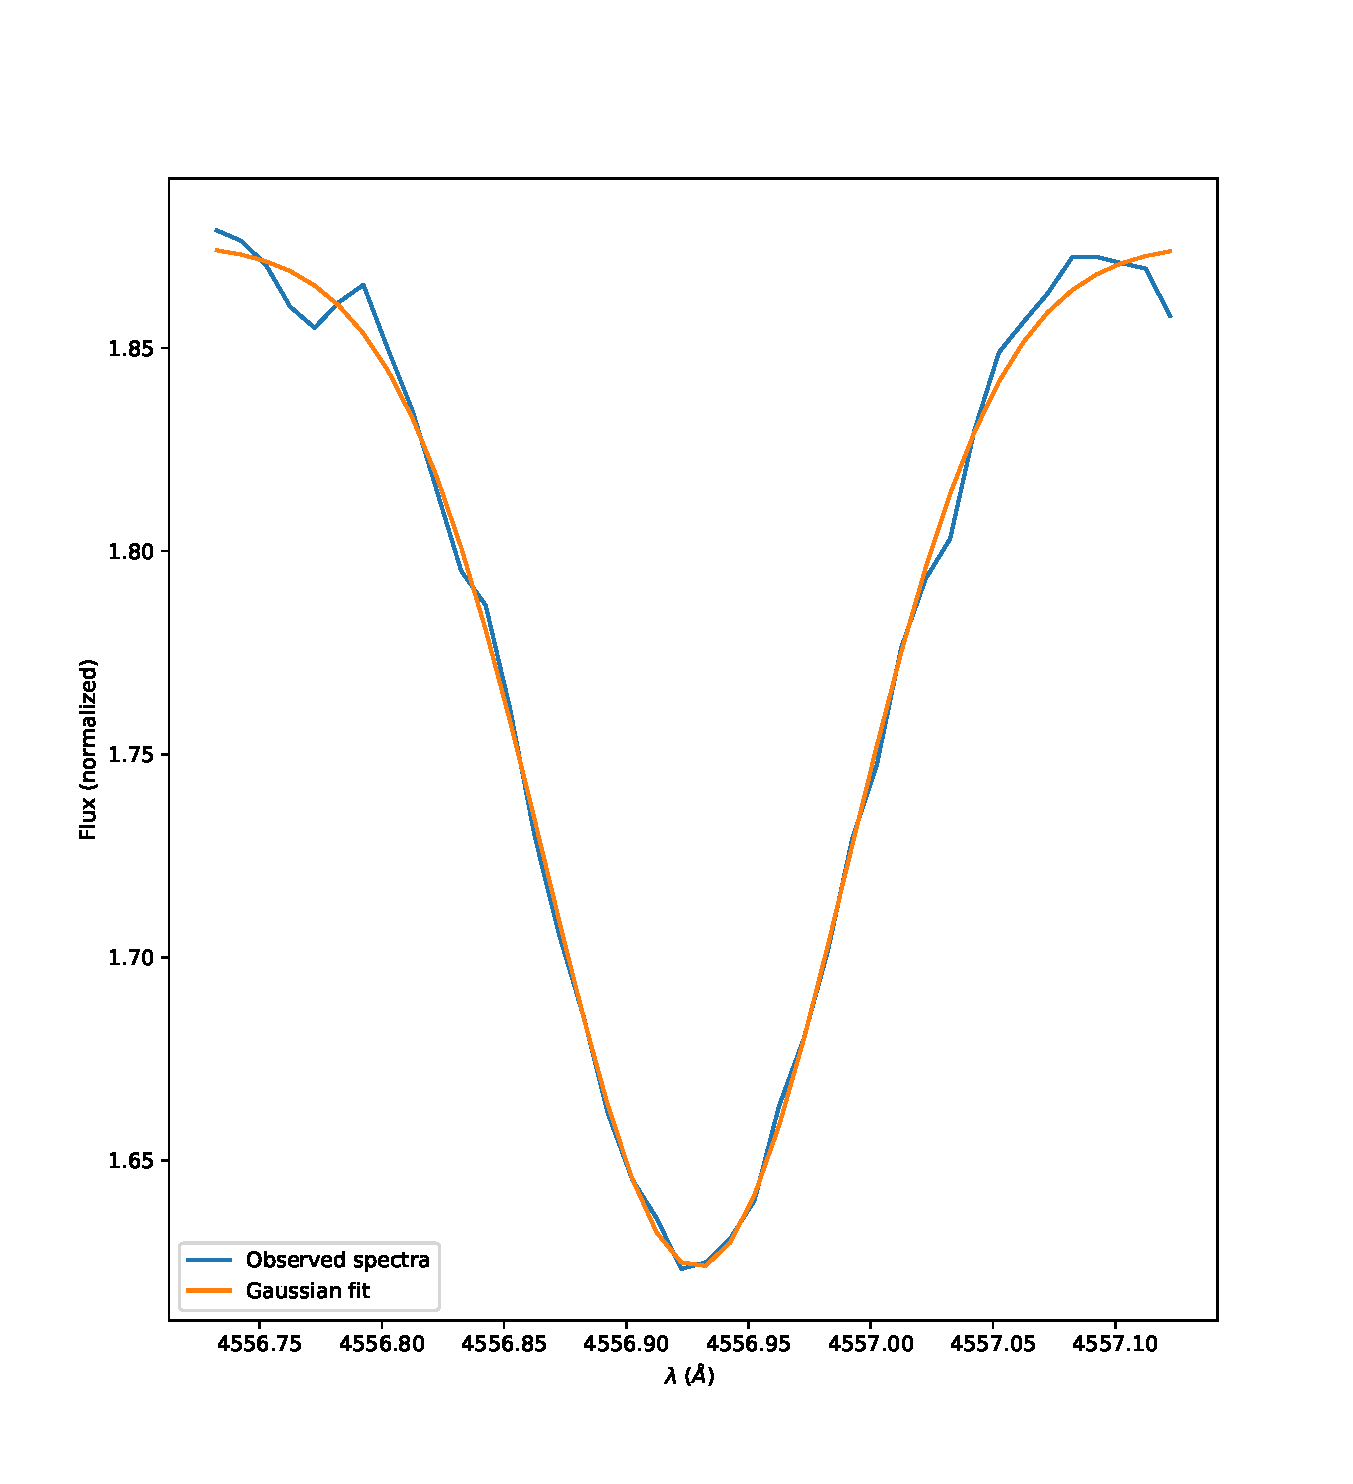
\includegraphics[width=\linewidth]{line_fit1.pdf}
  \caption{Gaussian fit to spectral line}
  \label{fig:line_fit}
\end{figure}

\subsection{Temperature estimation}

With efficiency in mind, we start by estimating the effective temperature of our
spectra, as this allows us to limit the range of spectra to lookup in the
database greatly. We achieve this by calculating the equivalent width of lines
of two multiplets of sufficiently different excitation energy and plotting
$log \left(  W / \lambda \right)$ by $\log \left( g f \lambda \right)$. From the
relation (\cite{monteiro_sebenta_2019}) 

\begin{equation}
  \label{eq:log_W_relation}
  \log \left( \frac{W_\lambda}{\lambda} \right) = \alpha  + \log \left( \lambda f_i g_i \right) - \frac{5040}{T_{\text{exc}}} \chi_i
\end{equation}

with $\log \left( \lambda f_i g_i \right)$ and $\chi_i$ know for each multiplet
(\cite{tsantaki_deriving_2013}), and $\alpha$ a constant, we may denote the average distance between
linear fits (for which equation \ref{eq:log_W_relation} is common) as $\Delta$ and obtain

\begin{equation}
  \label{eq:T_exc}
  T_{\text{exc}} = \frac{| 5040 \left( \chi_2 - \chi_1 |\right)}{\Delta}
\end{equation}

Using known equivalent widths for the sun's lines (Figure \ref{fig:temp_estimation_sun})
we get $T = 5769$ K directly from equation \ref{eq:T_exc}.

\begin{figure}
  \centering
  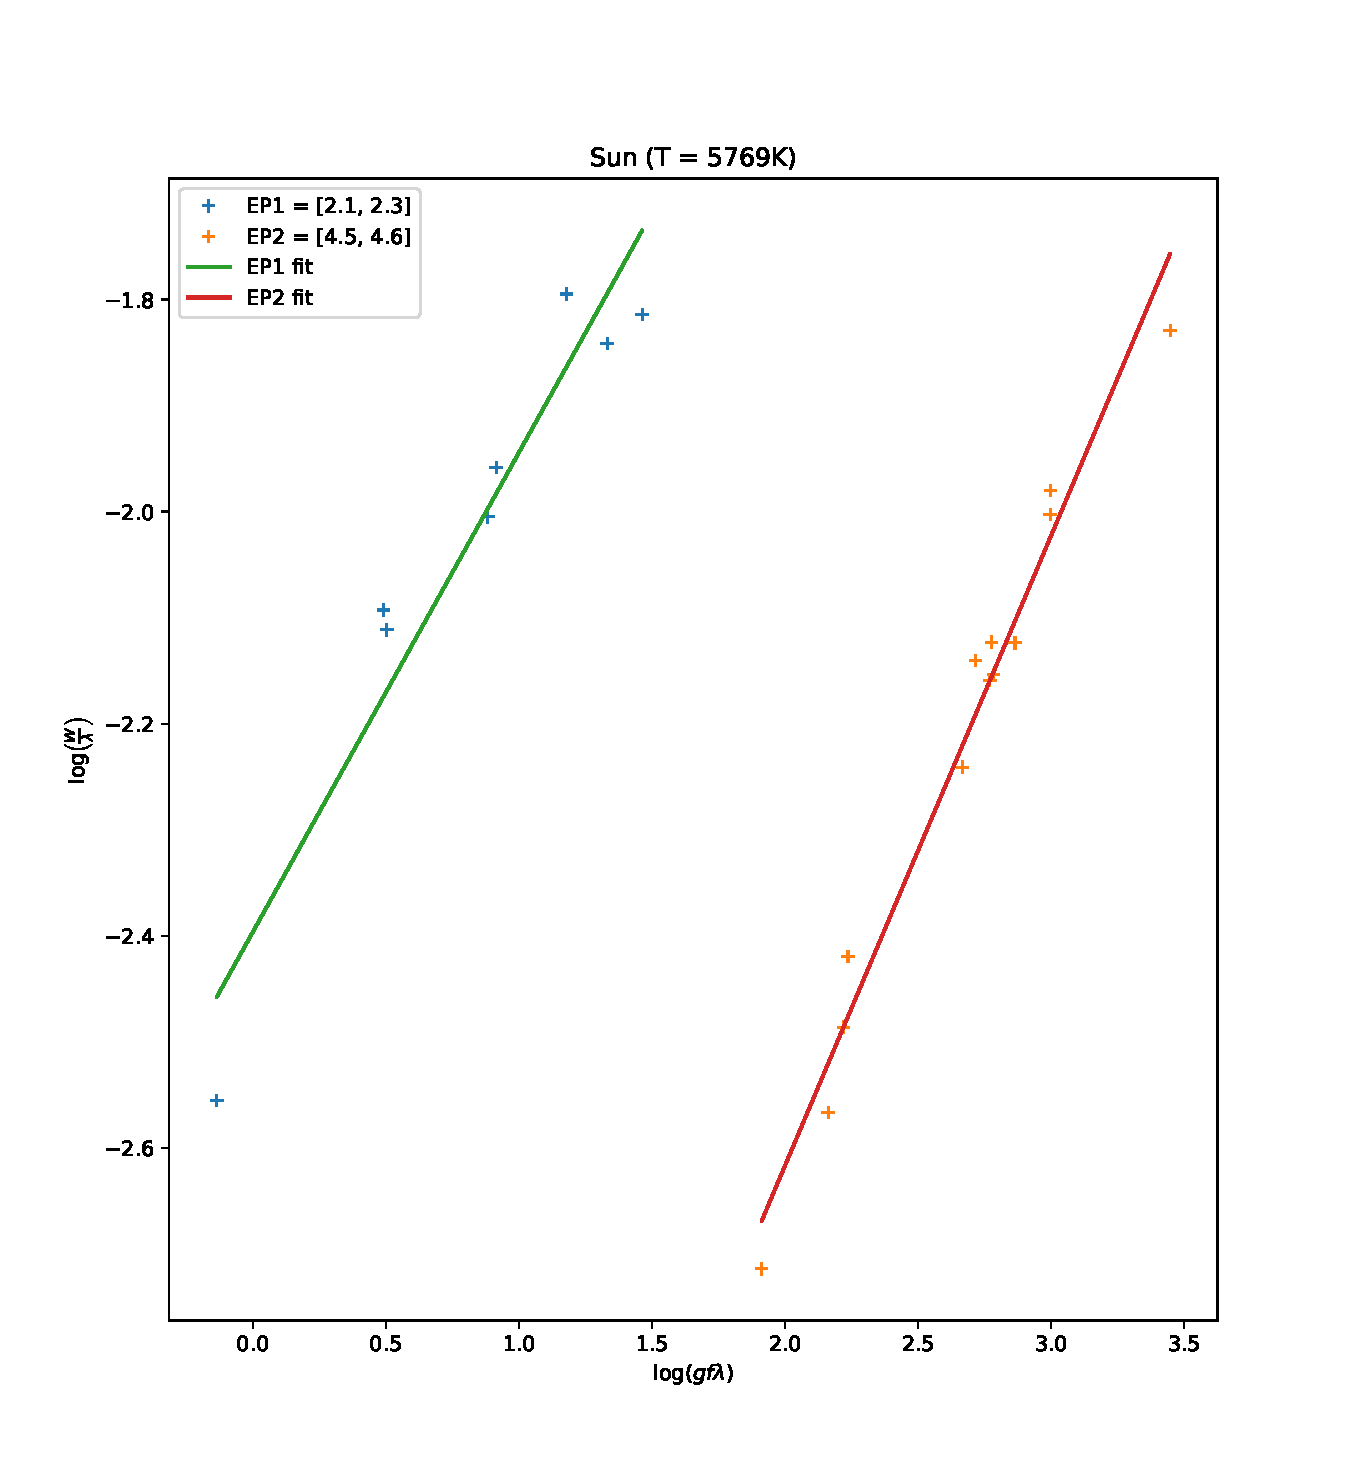
\includegraphics[width=\linewidth]{temperature_estimation_sun.pdf}
  \caption{Sun's temperature estimation}
  \label{fig:temp_estimation_sun}
\end{figure}

\subsection{Synthetic spectra database lookup and comparison}

Setting an uncertainty interval on the temperature $\Delta T$  (in our case,
$\Delta T$ = 400K), one may now compare the observed spectra with synthetic
spectra (in \cite{laverny_ambre_2012}) with temperatures in the range $T\in [T - \Delta T, T + \Delta T]$.

This comparison proceeds once again by calculating the equivalent width of known
lines of both spectra. We may then plot $W_\text{synt}$ by $W_\text{obs}$ and
determine the best synthetic spectra by determining the one
corresponding to a linear fit of slope closest to unity. \footnote{Alternatively, a least squares
  comparison may be used. The reasons for not using this method will be
  clarified later. They may nevertheless be reduced to equivalent methods,
  depending on the choice of lines. Due to the efficiency of computational
  fitting methods, there is no significant slowdown.}


\subsection{Synthetic spectra processing}

With the best fitting spectra found, one need only process it before the comparison
with the observed spectra. This consists of:

\begin{enumerate}
\item applying the experimental profile of
  the instrument of measurement used, by means of a convolution of the spectra
  with a Gaussian determined by the experimental parameters as in equation
  \ref{eq:exp_profile_params} (\cite{monteiro_sebenta_2019}).

  \begin{equation}
    \label{eq:exp_profile_params}
    \sigma = \frac{<\lambda>}{R \sqrt{8 \ln (2)}}
  \end{equation}

  being $\sigma$ the standard deviation of the Gaussian function and $R$ the
  resolution of the instrument ($R \approx 50000$ for HARPS used in \cite{tsantaki_deriving_2013}).

\item applying the rotational profile of the star by \#TODO
\item interpolating the synthetic spectra with observed data for ease of
  posterior analysis. 
\end{enumerate}



%-------------------------------------------------------------------
\section{Conclusions}

   \begin{enumerate}
      \item The conditions for the stability of static, radiative
         layers in gas spheres, as described by Baker's (\citeyear{baker})
         standard one-zone model, can be expressed as stability
         equations of state. These stability equations of state depend
         only on the local thermodynamic state of the layer.
      \item If the constitutive relations -- equations of state and
         Rosseland mean opacities -- are specified, the stability
         equations of state can be evaluated without specifying
         properties of the layer.
      \item For solar composition gas the $\kappa$-mechanism is
         working in the regions of the ice and dust features
         in the opacities, the $\mathrm{H}_2$ dissociation and the
         combined H, first He ionization zone, as
         indicated by vibrational instability. These regions
         of instability are much larger in extent and degree of
         instability than the second He ionization zone
         that drives the Cephe{\"\i}d pulsations.
   \end{enumerate}

\begin{acknowledgements}
      Part of this work was supported by the German
      \emph{Deut\-sche For\-schungs\-ge\-mein\-schaft, DFG\/} project
      number Ts~17/2--1.
\end{acknowledgements}

% WARNING
%-------------------------------------------------------------------
% Please note that we have included the references to the file aa.dem in
% order to compile it, but we ask you to:
%
% - use BibTeX with the regular commands:
%   \bibliographystyle{aa} % style aa.bst
%   \bibliography{Yourfile} % your references Yourfile.bib
%
% - join the .bib files when you upload your source files
%-------------------------------------------------------------------

\bibliographystyle{aa}
\bibliography{spectra}

\end{document}